\chapter{Testbed}
\label{chap:testbed}
After introducing relevant background and presenting related works that this research paper builds upon in the State-of-the-Art chapter~\ref{chap:sota}, the testbed chapter introduces relevant terms to testing the architecture designed and implemented in the previous system design chapter~\ref{chap:design}. Following the introduction of basic terms necessary to understand the impetus of the testbed, this chapter details the hardware upon which GNL was tested, as well as the instrumentation methodology. Lastly, this chapter summarizes the different experiments devised to evaluate the implementation of GNL.

\section{Wireless Opportunistic Networks as a Bridge to Collective Communication}
Collective Communication is a distributed computing term, in which a group of participating nodes communicate and coordinate to jointly compute a shared difficult task. In collective communication, a set of standard collective operations is identified and derived from complex tasks, to compute the processing of sub-tasks whose results will get aggregated and often distributed. A classic analogy of collective communication from the real-world is the counting of election votes. Deciding which candidate has the most vote can be efficiently broken down to individual tasks that may be computed in parallel: counting the votes each candidate received in each voting station, aggregating the results of different stations in a single city, aggregating different cities into regions, before finally summing tallied regional votes into a final national vote to decide the election. Moving to the digital realm, this analogy can be realized with a concrete example. As machine learning and other AI models usage rocketed, more weakness points in their design and implementation began to surface. Most prominently, their training process is highly centralized which requires a massive amount of data and processing power, and presents a single point of failure; training is mostly conducted on cloud servers residing in data centers, which also exposes privacy concerns due to the transport of personal data to data centers, which often reside on a different continent~\cite{Moussa2025}. These outlined issues incentivize exploring neighborhood data centers as a form of community hyper-scalars, to maintain data processing with data origin. To do that, processing units of co-located across different devices can be combined, like smartphones, personal computers, and other IoT edge devices. The hybrid processing environment and diverse network topologies present when combining a variety of devices presents itself as a real obstacle in tapping this source of computing power. To overcome this obstacle, OppNets can be used to bypass the need for a strict end-to-end path, and exploiting the physical proximity between users, direct p2p protocols such as Bluetooth may be used as a transport substrate to facilitate communication and enable more performant transport channels.
Building upon the GNL system architecture introduced in section~\ref{sec:system-arch}, this section explores the execution of collective communication operations on an OppNet-based app. Traditionally relying on stable network topologies with constantly available end-to-end paths, this research work explores the execution of those operations on an opportunistic network to coordinate distributed processing on edge devices. Ultimately, this architectural foundation empowers communities to use infrastructure-free, self-owned data centers by providing mechanisms necessary to support a resilient collective data exchange across unpredictable OppNets.

\subsection{Fundamentals of Collective Communication}
Extensive algorithmic and analytical research has established a set of fundamental collective-communication operations: Broadcast, Reduce, All-Reduce, Scatter, Gather, All-Gather and All-to-All~\cite{Sanders2019}.
These operations are used to model information flow in collective communication networks like parallelized, distributed systems:\begin{itemize}
\item \emph{Broadcast}: The Broadcast operation models a single node sending a copy of its message to all other nodes in the network.
\item \emph{Reduce}: One message from each node is combined into a single result using an associative operator such as addition, and delivered to a single node.
\item \emph{All-Reduce}: A combination of reduce and broadcast, where the final combined result is then broadcast to all nodes.
\item \emph{Scatter}: The Scatter operation models a single node distributing a distinct individual message to all other nodes.
\item \emph{Gather}: The Gather operation models all nodes uniting their message to a single, concatenated message, which then gets sent to one node.
\item \emph{All-Gather}: A combination of Gather and Broadcast, where the final concatenated result is then broadcast to all nodes.
\item \emph{All-to-All}: The All-to-All broadcast has every node broadcast a distinct, individual message to every other node.
\end{itemize}
To better understand the clash between parallel processing algorithms that require highly-regular interaction patterns with low-level communication mediums (e.g. antennas) present on standard machines, these models were standardized into a set to help research simplify complex parallel computing tasks.
The collective communication operations are traditionally modeled and evaluated mathematically across different network topologies, including \emph{line},\emph{tree},hyper-\emph{cube} toppologies.
While there is no shortage of analytical results and proven analytical bounds for these operations (e.g. calculating transmission costs), these research works are mostly constrained to predicted, stable networks and synchronized parallel computing environments. There is a paradigm shift required to adapt these operations to OppNets, as they require mainly synchronous execution over rigid geometric topologies: the research community began mapping those operations to physical mobile devices by using asynchronous delay-tolerant mechanisms: Store-Carry-Forward in all-to-all broadcast epidemic routing, CRDTs for global state synchronization instead of consensus, and federated learning for an all-reduce computation~\cite{Maheo2023,TranTruong2026}. This testbed evaluates how effectively we can map these collective operations onto the physical world, using an 8-device mesh, simulating different network topologies and movement models. To evaluate the system architecture, we deployed the dummy mobile application on a limited testbed of Android and iOS devices, and uploaded the trace resulting from the experiments to a server. Before evaluating network-layer behavior, we characterize the radio link itself: at what signal strength a link between two devices can be discovered, established, and used, and what data rate it sustains as it degrades. These two experiments provide the physical-layer baseline that the distances and placements of all subsequent experiments build upon.

\section{Control plane: RSSI and link establishment on a line}

\paragraph{Question.} At what received signal strength does a link between two peers
become discoverable, established, and usable --- and how many bytes does the control
plane expose on the air to establish a link and keep it alive?

\paragraph{Setup.} Two nodes on stands at fixed height, open field with clear line of
sight. The nodes start $\sim$120\,m apart, beyond radio range, and are brought closer
in fixed steps down to 10\,m.

\paragraph{Procedure.} At each distance step the nodes dwell for several minutes,
sampling RSSI and recording link-establishment attempts, before moving to the next
step. The sweep is run in both directions --- approaching (no link $\to$ link) and
retreating (link $\to$ drop) --- to capture the hysteresis between the signal strength
required to \emph{form} a link and that required to \emph{keep} it. We distinguish
three link stages, which are expected to occur at different RSSI thresholds:
\begin{enumerate}
    \item \emph{Discovered}: a peer advertisement (ANNOUNCE) is received;
    \item \emph{Established}: the connection and handshake complete;
    \item \emph{Usable}: a first payload is delivered and acknowledged end-to-end.
\end{enumerate}

\paragraph{Measures.} Per-sample RSSI with ground-truth distance; timestamps of the
three link stages per attempt; control-plane bytes on the air (ANNOUNCE, handshake,
keepalive traffic) during establishment and during a steady link.

\paragraph{Output.} RSSI vs.\ distance with a log-distance path-loss fit;
link-establishment probability and stage breakdown per distance; establishment vs.\
drop threshold (hysteresis); control-plane cost in exposed bytes to establish a link
and to keep it alive per unit time.

\paragraph{Results.} Ten distances from 10\,m to 100\,m, ten trials each, on the
open field. Mean advertisement RSSI follows a log-distance law with exponent
$n=3.23$ and a residual standard deviation of 2.8\,dB:
%
\begin{equation}
  \mathrm{RSSI}(d) = -30.0 - 10\,n \log_{10} d, \qquad n = 3.23 .
  \label{eq:pathloss}
\end{equation}
%
An exponent above the free-space value of 2 is expected for antennas near
ground level, where the ground-reflected ray interferes with the direct one.

The central result is that the three link stages do \emph{not} share a range.
Table~\ref{tab:line-stages} gives the per-distance rates. Discovery, connection
and session track each other almost exactly --- a peer that is heard is a peer
that can be handshaked --- and all three survive to 90\,m at reduced
reliability. Sustained delivery does not: it is already eroding at 50\,m, where
every trial still reaches a session but only 74\% of messages arrive, and by
70\,m a session forms in 9 trials out of 10 while delivery has collapsed to
13\%. \emph{Maximum range therefore depends on the criterion.} Taking
establishment as the test puts the edge near 90\,m; taking sustained delivery
puts it between 40 and 50\,m. The gap between those two numbers is the region
where a pair repeatedly forms sessions it cannot use.

Latency degrades over the same interval rather than at the edge: the median
round trip is 181\,ms at 10\,m, 2.8\,s at 50\,m, 8.1\,s at 70\,m and 11.8\,s at
90\,m. The 100\,m step produced no discovery at all in any trial.

\begin{table}[t]
  \centering
  \small
  \caption[Link stage rates against distance]{%
    Per-distance stage rates, ten trials each, approaching. \emph{Session} is a
    completed Noise handshake; \emph{usable} additionally requires a payload
    delivered and acknowledged end to end. Delivery is the fraction of sent
    messages that arrived; RTT is the median round trip.}
  \label{tab:line-stages}
  \begin{tabular}{@{}rrrrrrr@{}}
    \toprule
    $d$ (m) & RSSI (dBm) & disc. & sess. & usable & delivery & RTT (ms) \\
    \midrule
    10  & $-60.0$ & 1.00 & 1.00 & 1.00 & 1.00 & 181 \\
    20  & $-69.3$ & 1.00 & 1.00 & 1.00 & 1.00 & 665 \\
    30  & $-80.7$ & 1.00 & 1.00 & 1.00 & 1.00 & 227 \\
    40  & $-85.1$ & 1.00 & 1.00 & 0.90 & 0.90 & 247 \\
    50  & $-87.6$ & 1.00 & 1.00 & 1.00 & 0.74 & 2801 \\
    60  & $-91.1$ & 0.90 & 0.90 & 0.60 & 0.77 & 996 \\
    70  & $-89.7$ & 0.90 & 0.90 & 0.30 & 0.13 & 8133 \\
    80  & $-91.5$ & 0.20 & 0.20 & 0.00 & 0.00 & --- \\
    90  & $-89.1$ & 0.50 & 0.40 & 0.10 & 0.25 & 11845 \\
    100 & $-91.3$ & 0.00 & 0.00 & 0.00 & --- & --- \\
    \bottomrule
  \end{tabular}
\end{table}

Pooled over all 100 trials the ladder loses most of its attrition at the last
rung: 75\% of trials discovered the peer, 74\% reached a session, and 59\%
became usable. Median time to discovery is 3.2\,s and to a session 6.3\,s, but
the 90th percentile is 20.6\,s and 25.5\,s --- the distribution has a long tail
even where the link ultimately forms.

\paragraph{Control-plane cost.} Establishing and holding a link is cheap for
the protocol and expensive for the radio. Over a 30\,s dwell at 10\,m the
protocol put $\sim$2.3\,kB of ANNOUNCE and 0.37\,kB of handshake on the air,
against $\sim$51\,kB of OS advertising emitted by the controller below the
application over the same window --- computed from the measured 21-byte
advertisement payload on three primary channels at the measured 130\,ms
interval. \textbf{More than 94\% of control-plane airtime is the
advertisement, not the protocol.} The protocol's own share falls with distance
only because fewer peers are heard to answer; the advertising cost is constant
and is paid whether or not anyone is listening.

Power over the same session was 348\,mA on the moving node and 380\,mA on the
static one, projecting to roughly 7--8 hours of continuous operation on the
2700\,mAh handsets used.

\begin{figure}[t]
  \centering
  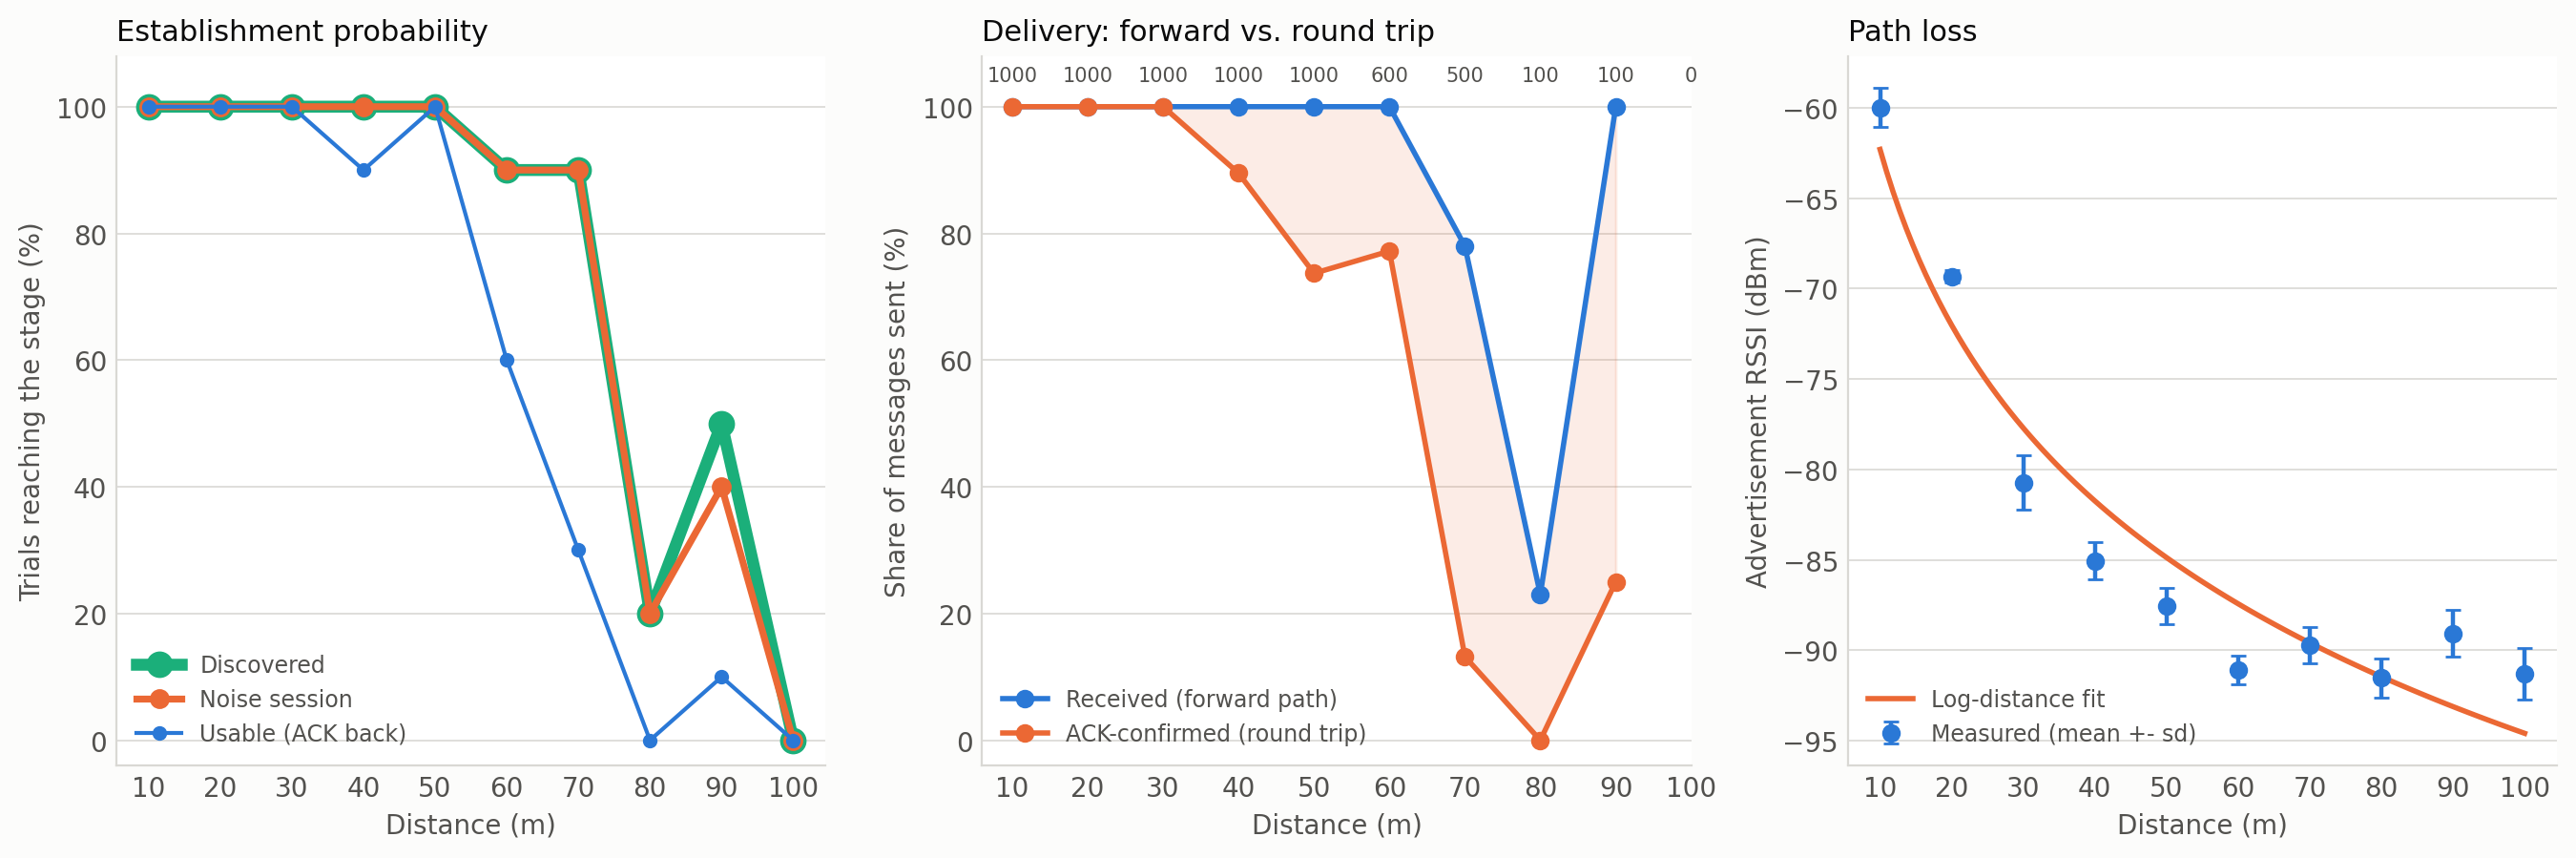
\includegraphics[width=\linewidth]{figures/line_experiment.png}
  \caption[The line experiment]{%
    Establishment probability and delivery against distance with the
    path-loss fit of Eq.~\eqref{eq:pathloss}. The separation between the
    establishment curve and the delivery curve is the usable-range gap.}
  \label{fig:line-experiment}
\end{figure}

\begin{figure}[t]
  \centering
  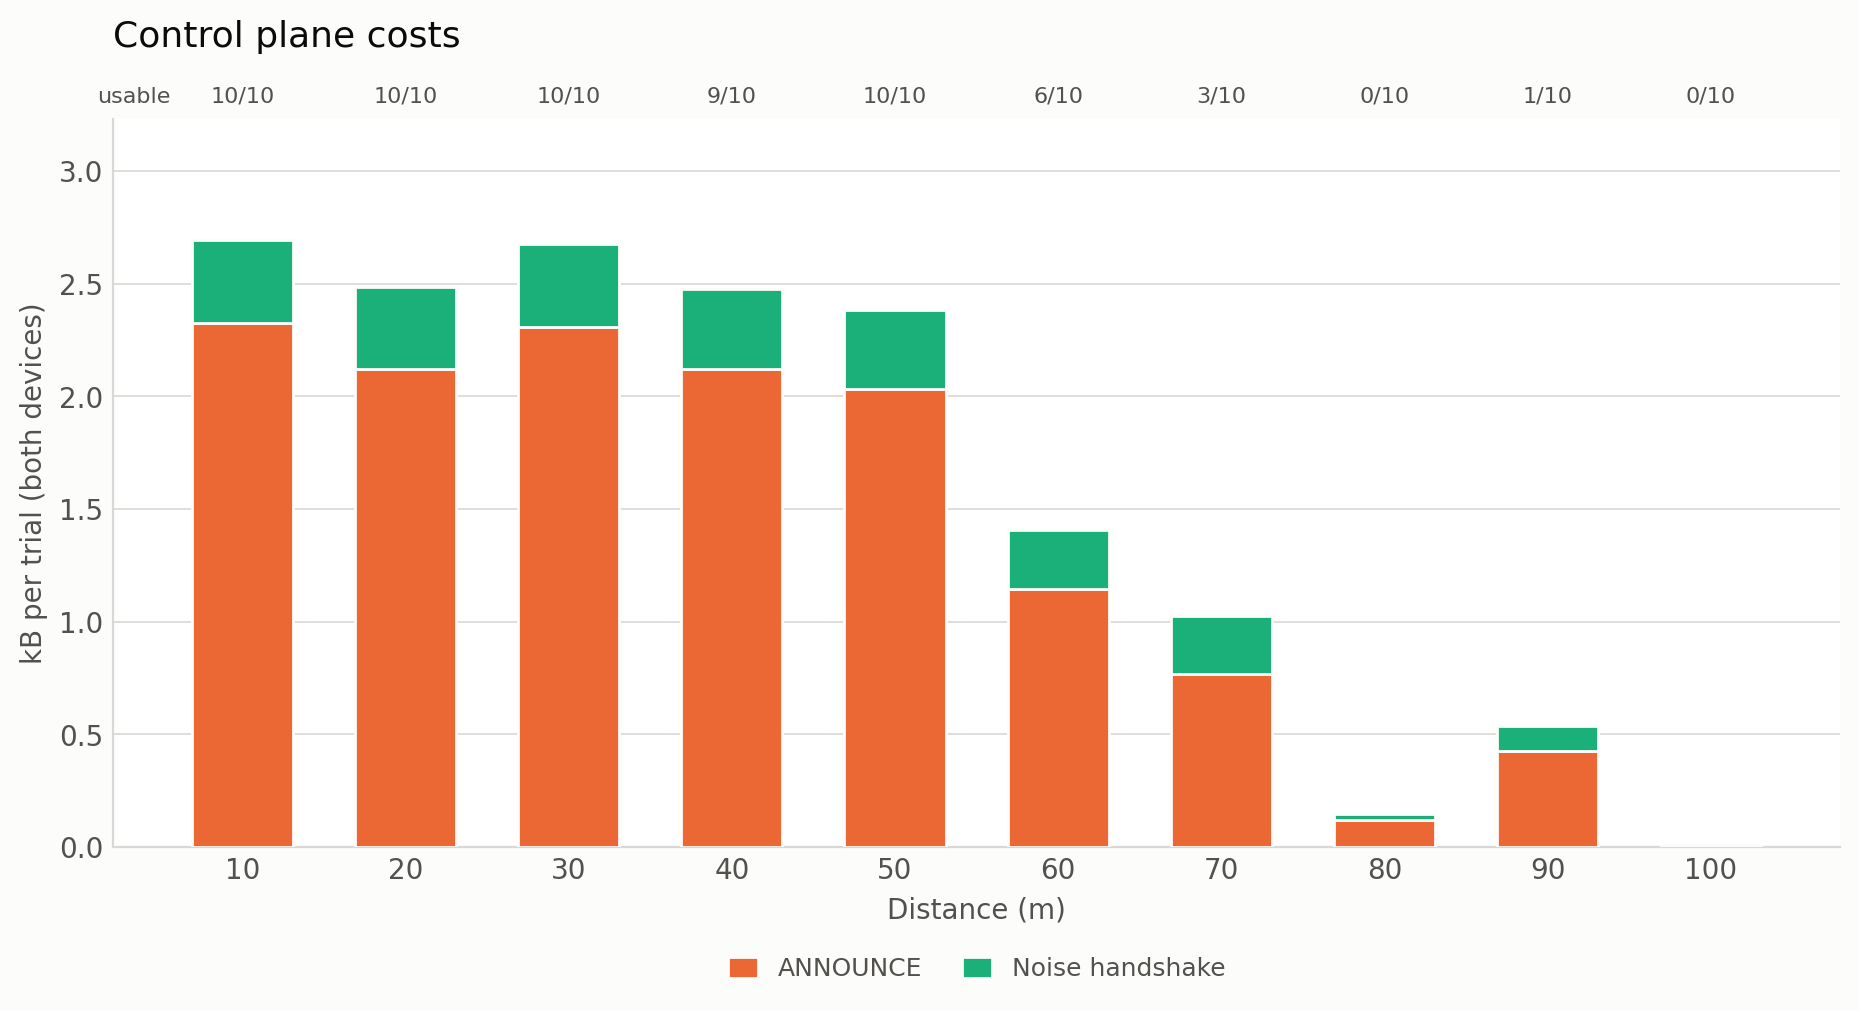
\includegraphics[width=\linewidth]{figures/line_establish_bytes.png}
  \caption[Control-plane bytes per distance]{%
    Bytes on the air per 30\,s dwell, split into what the protocol sends and
    what the OS advertiser sends regardless of it.}
  \label{fig:line-bytes}
\end{figure}

\section{Data plane: throughput of a dilating clique}

\paragraph{Question.} How does the achievable throughput of a fully-connected clique
degrade as the area it covers grows --- i.e., how much ground can a clique cover
before its capacity collapses?

\paragraph{Setup.} Three nodes positioned in an equilateral triangle. The side length
is increased step-wise, uniformly dilating the clique from close proximity up to the
link-drop distance established in the control-plane experiment.

\paragraph{Procedure.} At each side length, first a pairwise single-flow transfer
between two nodes establishes the distance-only baseline; then all three pairs run
simultaneous transfers (all-to-all workload). Transfers use large, fragmented
payloads so that each measurement window captures sustained throughput. The
difference between the baseline and the simultaneous runs isolates the cost of
medium contention from the cost of distance.

\paragraph{Measures.} Per-link RSSI; per-flow goodput; end-to-end latency; delivery
failures per side length.

\paragraph{Output.} Throughput vs.\ RSSI and vs.\ side length, single-flow and
contended; aggregate clique throughput vs.\ covered area, showing how capacity
changes as the clique dilates.

\begin{table}[t]
  \centering
  \small
  % \caption[Testbed hardware]
  % \label{tab:testbed-hardware}
  \begin{tabular}{@{}clllc@{}}
    \toprule
    \textbf{Units} & \textbf{Device} & \textbf{SoC} & \textbf{OS} & \textbf{BT} \\
    \midrule
    \multicolumn{5}{@{}l}{} \\
    4 & LG Nexus 5X       & Snapdragon 808 & Android 8.1 & 4.2 \\
    1 & Samsung Galaxy S10e & Exynos 9820  & Android 12  & 5.0 \\
    1 & Huawei Mate 20    & Kirin 980      & Android 9   & 5.0 \\
    1 & Google Pixel 2    & Snapdragon 835 & Android 11  & 5.0 \\
    1 & Google Pixel 10 Pro & Tensor G5    & Android 16  & 6.0 \\
    1 & Samsung Galaxy A72 & Snapdragon 720G & Android 14 & 5.0 \\
    1 & Samsung Galaxy Note20 & Exynos 990 & Android 13  & 5.0 \\
    1 & Google Pixel 7a   & Tensor G2      & Android 15  & 5.3 \\
    1 & Apple iPhone \textit{TBD} & \textit{TBD} & iOS \textit{TBD} & \textit{TBD} \\
    1 & Apple iPad \textit{TBD}   & \textit{TBD} & iPadOS \textit{TBD} & \textit{TBD} \\
    \bottomrule
  \end{tabular}
\end{table}
